% Options for packages loaded elsewhere
\PassOptionsToPackage{unicode}{hyperref}
\PassOptionsToPackage{hyphens}{url}
%
\documentclass[
  a4paper,
]{book}
\usepackage{amsmath,amssymb}
\usepackage{lmodern}
\usepackage{ifxetex,ifluatex}
\ifnum 0\ifxetex 1\fi\ifluatex 1\fi=0 % if pdftex
  \usepackage[T1]{fontenc}
  \usepackage[utf8]{inputenc}
  \usepackage{textcomp} % provide euro and other symbols
\else % if luatex or xetex
  \usepackage{unicode-math}
  \defaultfontfeatures{Scale=MatchLowercase}
  \defaultfontfeatures[\rmfamily]{Ligatures=TeX,Scale=1}
\fi
% Use upquote if available, for straight quotes in verbatim environments
\IfFileExists{upquote.sty}{\usepackage{upquote}}{}
\IfFileExists{microtype.sty}{% use microtype if available
  \usepackage[]{microtype}
  \UseMicrotypeSet[protrusion]{basicmath} % disable protrusion for tt fonts
}{}
\makeatletter
\@ifundefined{KOMAClassName}{% if non-KOMA class
  \IfFileExists{parskip.sty}{%
    \usepackage{parskip}
  }{% else
    \setlength{\parindent}{0pt}
    \setlength{\parskip}{6pt plus 2pt minus 1pt}}
}{% if KOMA class
  \KOMAoptions{parskip=half}}
\makeatother
\usepackage{xcolor}
\IfFileExists{xurl.sty}{\usepackage{xurl}}{} % add URL line breaks if available
\IfFileExists{bookmark.sty}{\usepackage{bookmark}}{\usepackage{hyperref}}
\hypersetup{
  pdftitle={MATH1710 Probability and Statistics I},
  pdfauthor={Matthew Aldridge},
  hidelinks,
  pdfcreator={LaTeX via pandoc}}
\urlstyle{same} % disable monospaced font for URLs
\usepackage{color}
\usepackage{fancyvrb}
\newcommand{\VerbBar}{|}
\newcommand{\VERB}{\Verb[commandchars=\\\{\}]}
\DefineVerbatimEnvironment{Highlighting}{Verbatim}{commandchars=\\\{\}}
% Add ',fontsize=\small' for more characters per line
\usepackage{framed}
\definecolor{shadecolor}{RGB}{248,248,248}
\newenvironment{Shaded}{\begin{snugshade}}{\end{snugshade}}
\newcommand{\AlertTok}[1]{\textcolor[rgb]{0.94,0.16,0.16}{#1}}
\newcommand{\AnnotationTok}[1]{\textcolor[rgb]{0.56,0.35,0.01}{\textbf{\textit{#1}}}}
\newcommand{\AttributeTok}[1]{\textcolor[rgb]{0.77,0.63,0.00}{#1}}
\newcommand{\BaseNTok}[1]{\textcolor[rgb]{0.00,0.00,0.81}{#1}}
\newcommand{\BuiltInTok}[1]{#1}
\newcommand{\CharTok}[1]{\textcolor[rgb]{0.31,0.60,0.02}{#1}}
\newcommand{\CommentTok}[1]{\textcolor[rgb]{0.56,0.35,0.01}{\textit{#1}}}
\newcommand{\CommentVarTok}[1]{\textcolor[rgb]{0.56,0.35,0.01}{\textbf{\textit{#1}}}}
\newcommand{\ConstantTok}[1]{\textcolor[rgb]{0.00,0.00,0.00}{#1}}
\newcommand{\ControlFlowTok}[1]{\textcolor[rgb]{0.13,0.29,0.53}{\textbf{#1}}}
\newcommand{\DataTypeTok}[1]{\textcolor[rgb]{0.13,0.29,0.53}{#1}}
\newcommand{\DecValTok}[1]{\textcolor[rgb]{0.00,0.00,0.81}{#1}}
\newcommand{\DocumentationTok}[1]{\textcolor[rgb]{0.56,0.35,0.01}{\textbf{\textit{#1}}}}
\newcommand{\ErrorTok}[1]{\textcolor[rgb]{0.64,0.00,0.00}{\textbf{#1}}}
\newcommand{\ExtensionTok}[1]{#1}
\newcommand{\FloatTok}[1]{\textcolor[rgb]{0.00,0.00,0.81}{#1}}
\newcommand{\FunctionTok}[1]{\textcolor[rgb]{0.00,0.00,0.00}{#1}}
\newcommand{\ImportTok}[1]{#1}
\newcommand{\InformationTok}[1]{\textcolor[rgb]{0.56,0.35,0.01}{\textbf{\textit{#1}}}}
\newcommand{\KeywordTok}[1]{\textcolor[rgb]{0.13,0.29,0.53}{\textbf{#1}}}
\newcommand{\NormalTok}[1]{#1}
\newcommand{\OperatorTok}[1]{\textcolor[rgb]{0.81,0.36,0.00}{\textbf{#1}}}
\newcommand{\OtherTok}[1]{\textcolor[rgb]{0.56,0.35,0.01}{#1}}
\newcommand{\PreprocessorTok}[1]{\textcolor[rgb]{0.56,0.35,0.01}{\textit{#1}}}
\newcommand{\RegionMarkerTok}[1]{#1}
\newcommand{\SpecialCharTok}[1]{\textcolor[rgb]{0.00,0.00,0.00}{#1}}
\newcommand{\SpecialStringTok}[1]{\textcolor[rgb]{0.31,0.60,0.02}{#1}}
\newcommand{\StringTok}[1]{\textcolor[rgb]{0.31,0.60,0.02}{#1}}
\newcommand{\VariableTok}[1]{\textcolor[rgb]{0.00,0.00,0.00}{#1}}
\newcommand{\VerbatimStringTok}[1]{\textcolor[rgb]{0.31,0.60,0.02}{#1}}
\newcommand{\WarningTok}[1]{\textcolor[rgb]{0.56,0.35,0.01}{\textbf{\textit{#1}}}}
\usepackage{longtable,booktabs,array}
\usepackage{calc} % for calculating minipage widths
% Correct order of tables after \paragraph or \subparagraph
\usepackage{etoolbox}
\makeatletter
\patchcmd\longtable{\par}{\if@noskipsec\mbox{}\fi\par}{}{}
\makeatother
% Allow footnotes in longtable head/foot
\IfFileExists{footnotehyper.sty}{\usepackage{footnotehyper}}{\usepackage{footnote}}
\makesavenoteenv{longtable}
\usepackage{graphicx}
\makeatletter
\def\maxwidth{\ifdim\Gin@nat@width>\linewidth\linewidth\else\Gin@nat@width\fi}
\def\maxheight{\ifdim\Gin@nat@height>\textheight\textheight\else\Gin@nat@height\fi}
\makeatother
% Scale images if necessary, so that they will not overflow the page
% margins by default, and it is still possible to overwrite the defaults
% using explicit options in \includegraphics[width, height, ...]{}
\setkeys{Gin}{width=\maxwidth,height=\maxheight,keepaspectratio}
% Set default figure placement to htbp
\makeatletter
\def\fps@figure{htbp}
\makeatother
\setlength{\emergencystretch}{3em} % prevent overfull lines
\providecommand{\tightlist}{%
  \setlength{\itemsep}{0pt}\setlength{\parskip}{0pt}}
\setcounter{secnumdepth}{5}
\usepackage{booktabs}
\ifluatex
  \usepackage{selnolig}  % disable illegal ligatures
\fi
\usepackage[]{natbib}
\bibliographystyle{plainnat}

\title{MATH1710 Probability and Statistics I}
\author{\href{mailto:math1710@leeds.ac.uk}{Matthew Aldridge}}
\date{University of Leeds, 2021--22}

\usepackage{amsthm}
\newtheorem{theorem}{Theorem}[chapter]
\newtheorem{lemma}{Lemma}[chapter]
\newtheorem{corollary}{Corollary}[chapter]
\newtheorem{proposition}{Proposition}[chapter]
\newtheorem{conjecture}{Conjecture}[chapter]
\theoremstyle{definition}
\newtheorem{definition}{Definition}[chapter]
\theoremstyle{definition}
\newtheorem{example}{Example}[chapter]
\theoremstyle{definition}
\newtheorem{exercise}{Exercise}[chapter]
\theoremstyle{definition}
\newtheorem{hypothesis}{Hypothesis}[chapter]
\theoremstyle{remark}
\newtheorem*{remark}{Remark}
\newtheorem*{solution}{Solution}
\begin{document}
\maketitle

{
\setcounter{tocdepth}{1}
\tableofcontents
}
\hypertarget{schedule}{%
\chapter*{Schedule}\label{schedule}}
\addcontentsline{toc}{chapter}{Schedule}

\textbf{Week 1} (27 September -- 1 October):

\begin{itemize}
\tightlist
\item
  \protect\hyperlink{S01-eda}{\textbf{Section 1:} Exploratory data analysis}
\item
  \protect\hyperlink{P1}{\textbf{Problem Sheet 1:}} all questions -- deadline for assessed questions: Monday 11 October
\item
  \protect\hyperlink{r-work}{\textbf{R Worksheet 1}}
\end{itemize}

\hypertarget{about}{%
\chapter*{About MATH1710}\label{about}}
\addcontentsline{toc}{chapter}{About MATH1710}

\hypertarget{organisation}{%
\section*{Organisation of MATH1710}\label{organisation}}
\addcontentsline{toc}{section}{Organisation of MATH1710}

This module is \textbf{MATH1710 Probability and Statistics I}. A few students will be taking this module as half of \textbf{MATH2700 Probability and Statistics for Scientists}.

This module lasts for 11 weeks from 27 September to 10 December 2021. The exam will take place between 10 and 21 January 2022.

The core teaching team are:

\begin{itemize}
\tightlist
\item
  Dr Matthew Aldridge (you can call me ``Matt'' or ``Dr Aldridge''): I am the module leader, the main lecturer, and the main author of these notes.
\item
  A module assistant TBC.
\end{itemize}

The shared email address for the core teaching team is \href{mailto:math1710@leeds.ac.uk}{\nolinkurl{math1710@leeds.ac.uk}}; please use this address, rather than emailing our personal addresses; this will ensure your email is seen as soon as possible.

\hypertarget{notes}{%
\subsection*{Notes and videos}\label{notes}}
\addcontentsline{toc}{subsection}{Notes and videos}

The main way you will learn new material for this module is by reading these notes and by watching the accompanying pre-recorded videos. There will be one section of notes each week, for a total of 11 sections, with the final section being a summary and revision.

Reading mathematics is a slow process. Each section should take one and a half to two hours to work through; we recommend you split this into two or more sessions. If you find yourself regularly getting through sections in much less than that amount of time, you're probably not reading carefully enough through each sentence of explanation and each line of mathematics, including understanding the motivation, checking the accuracy, and making your own notes.

You are probably reading the web version of the notes. If you want a PDF or ebook copy (to read offline or to print out), they can be downloaded via the top ribbon of the page. (Warning: I have not made as much effort to make the PDF and ebook as neat and tidy as I have the web version, and there may be formatting errors.)

We are very keen to hear about errors in the notes mathematical, typographical or otherwise. Please, please \href{mailto:math1710@leeds.ac.uk}{email us} if think you may have found any.

\hypertarget{problem-sheets}{%
\subsection*{Problem sheets}\label{problem-sheets}}
\addcontentsline{toc}{subsection}{Problem sheets}

There will be 5 problem sheets. Each problem sheet has a number of short and long questions for you to cover in your own time to help you learn the material, and two assessed questions, which you should submit for marking. The assessed questions on each problem sheet make up 3\% of your mark on this module, for a total of 15\%. Although the deadlines are on Mondays, you are advised to complete and submit the work in the previous week.

\begin{longtable}[]{@{}ccc@{}}
\toprule
Problem Sheet & Sections covered & Assessed work due \\
\midrule
\endhead
1 & 1 & Monday 11 October (Week 3) \\
2 & 2 and 3 & Monday 25 October (Week 5) \\
3 & 4 and 5 & Monday 8 November (Week 7) \\
4 & 6 and 7 & Monday 22 November (Week 9) \\
5 & 8, 9 and 10 & Monday 6 December (Week 11) \\
\bottomrule
\end{longtable}

Assessed questions should be submitted in PDF format through Gradescope. (Further Gradescope details will follow.) Most students choose to hand-write their solutions and then scan them to PDF using their phone; you should use a proper scanning app -- we recommend Microsoft Office Lens or Adobe Scan -- and not just submit photographs.

\hypertarget{lectures}{%
\subsection*{Lectures}\label{lectures}}
\addcontentsline{toc}{subsection}{Lectures}

You will have one online synchronous (that is, live, not recorded) ``lecture'' session each week, with me, run through Zoom. Because this is a large cohort, we will split into two groups:

\begin{itemize}
\tightlist
\item
  Group 1: Mondays at 1200
\item
  Group 2: Mondays at 1500
\end{itemize}

You should check your timetable to see which lecture group you are in.

This will not be a ``lecture'' in the traditional sense of the term, but will be an opportunity to re-emphasise material you have already learned from notes and videos, to give extra examples, and to answer common student questions, with some degree of interactivity via quizzes, polls, and the chat box.

We will assume you have completed all the work for the previous week by the time of the lecture.

We are very keen to hear about things you'd like to go through in the lectures; please \href{mailto:math1710@leeds.ac.uk}{email us} with your suggestions.

\hypertarget{tutorials}{%
\subsection*{Tutorials}\label{tutorials}}
\addcontentsline{toc}{subsection}{Tutorials}

Tutorials are small groups of about a dozen students. You have been assigned to one of 38 tutorial groups, each with a member of staff as the tutor. Your tutorial group will meet five times, in Weeks 2, 4, 6, 8, and 10. Tutorial groups will meet in person on campus; you should check your timetable to see when and where your tutorial group meets. (For those not yet on campus, due to travel restrictions or health conditions, there will be an extra online tutorial group for the first few tutorials.)

The main goal of the tutorials will be to go over your answers to the non-assessed questions on the problems sheets in an interactive session. In this smaller group, you will be able to ask detailed questions of your tutor, and have the chance to discuss your answers to the problem sheet. Your tutor may ask you to present some of your work to your fellow students, or may give you the opportunity to work together with others during the tutorial. Your tutor may be willing to give you a hint on the assessed questions if you've made a first attempt but have got stuck.

My recommended approach to problem sheets and tutorials is the following:

\begin{itemize}
\tightlist
\item
  Work through the problem sheet before the tutorial, spending plenty of time on it, and making multiple efforts at questions you get stuck on. I recommend spending \emph{at least 3 hours per week} on the problem sheets, which will usually mean a total of \emph{at least 6 hours per problem sheet} (as most problem sheets cover two weeks). Collaboration is encouraged when working through the non-assessed problems, but I recommend writing up your work on your own; answers to assessed questions must be solely your own work.
\item
  Take advantage of the small group setting of the tutorial to ask for help or clarification on questions you weren't able to complete.
\item
  After the tutorial, attempt again the questions you were previously stuck on.
\item
  If you're still unable to complete a question after this second round of attempts, \emph{then} consult the solutions.
\end{itemize}

Your tutor will also be the marker of your answers to the assessed questions on the problem sheets.

\hypertarget{r-worksheets}{%
\subsection*{R worksheets}\label{r-worksheets}}
\addcontentsline{toc}{subsection}{R worksheets}

R is a programming language that is particularly good at working with probability and statistics. Learning to use R is an important part of this module, and is used in many other modules in the University, particularly in MATH1712 Probability and Statistics II. R is used by statisticians throughout academic and increasingly in industry too. Learning to program is a valuable skill for all students, and learning to use R is particularly valuable for students interested in statistics and related topics like actuarial science.

You will learn R by working through one R worksheet each week in your own time. Worksheets 3, 5, 7, 9 and 11 will also contain a couple of questions for assessment. Each of these is worth 3\% of your mark for a total of 15\%. I recommend spending one hour per week on the week's R worksheet, plus one extra hour if there are assessed questions that week.

You can read more about the language R, and about the program RStudio that we recommend you use to interact with R, in \protect\hyperlink{R}{the R section of these notes}.

To help you if you have problems with R, we have organised optional \textbf{R troubleshooting drop-in sessions}, where you can discuss any problems you have with an R expert, in Weeks 2 and 3. Check your timetable for details -- these will be listed on your timetable as ``practicals''.

\hypertarget{dropin}{%
\subsection*{Optional ``office hours'' drop-in sessions}\label{dropin}}
\addcontentsline{toc}{subsection}{Optional ``office hours'' drop-in sessions}

If you there is something in the module you wish to discuss privately one-on-one with the module core teaching team, the place for the is the optional weekly ``office hours'', which will operate as drop-in sessions. These sessions are an optional opportunity for you to ask questions you have to a member of staff; these are particularly useful if there's something on the module that you are stuck on or confused about, but we're happy to discuss any statistics-related issues or questions you have.

There will be two ``office hours'' drop-in sessions per week:

\begin{itemize}
\tightlist
\item
  Wednesday at 1000 in \href{https://ses.leeds.ac.uk/rooms?type=room\&id=1207583}{Charles Thackrah SR G.07}
\item
  Wednesday at 1200 in \href{https://students.leeds.ac.uk/rooms?type=room\&id=99930}{Emmanuel Centre SR 02}
\end{itemize}

(For timetabling reasons, the 1000 sessions appear on the timetable for MATH2700 students and the 1200 sessions appear on the timetable for MATH1710 students, but I'm happy for anyone to attend either hour.)

\hypertarget{time}{%
\subsection*{Time management}\label{time}}
\addcontentsline{toc}{subsection}{Time management}

It is, of course, up to you how you choose to spend your time on this module. But my recommendations for your weekly work would be something like this:

\begin{itemize}
\tightlist
\item
  \textbf{Notes and videos:} 2 hours per week/section
\item
  \textbf{Problem sheet:} 3 hours per week (so 6 hours for most problem sheets) plus 1 extra hour for writing up and submitting answers to assessed questions
\item
  \textbf{R worksheet:} 1 hour per week/worksheet, plus 1 extra hour if there are assessed questions
\item
  \textbf{Lecture:} 1 hour per week
\item
  \textbf{Tutorial:} 1 hour every other week
\item
  \textbf{Revision:} 13 hours total at the end of the module
\end{itemize}

That's roughly 8 hours a week, and makes 100 hours in total. (MATH1710 is a 10 credit module, so is supposed to represent 100 hours work. MATH2700 students are expected to be able to use their greater experience to get through the material in just 75 hours, so should scale these recommendations accordingly.)

\hypertarget{exam}{%
\subsection*{Exam}\label{exam}}
\addcontentsline{toc}{subsection}{Exam}

There will be an exam in January, which makes up the remaining 70\% of your mark. The exam will consist of 20 short and 2 long questions, and will be time-limited to 2 hours. We'll talk more about the exam format near the end of the module.

\hypertarget{ask}{%
\subsection*{Who should I ask about\ldots?}\label{ask}}
\addcontentsline{toc}{subsection}{Who should I ask about\ldots?}

Remember that the email address for the core module teaching team is \href{mailto:math1710@leeds.ac.uk}{\nolinkurl{math1710@leeds.ac.uk}}. Please don't email our personal addresses; it will take longer for us to reply, and we may miss your email all together.

\begin{itemize}
\tightlist
\item
  \emph{I don't understand something in the notes or on a problem sheet}: Come to office hours, or (if the timing works) ask your tutor in your next tutorial.
\item
  \emph{I'm having difficulties with R:} In Weeks 2 or 3, you should attend the R trouble-shooting drop-in session; at other times, come to office hours.
\item
  \emph{I have an admin question about arrangements for the module:} Come to office hours or \href{mailto:math1710@leeds.ac.uk}{email the core module teaching team}.
\item
  \emph{I have an admin question about arrangements for my tutorial:} Contact your tutor.
\item
  \emph{I have an admin question about general arrangements for my course as a whole:} \href{mailto:Maths.Taught.Students@leeds.ac.uk}{Email the Maths Taught Students Office (Maths.Taught.Students@leeds.ac.uk)} or speak to your personal academic tutor.
\item
  \emph{I have a question about the marking of my assessed work on the problem sheets:} First, check your feedback on Gradescope; if you still have questions, contact your tutor.
\item
  \emph{I have a question about the marking of my assessed work on the R worksheets:} Come to office hours or \href{mailto:math1710@leeds.ac.uk}{email the core module teaching team}.
\item
  \emph{I have suggestion for something to cover in the lectures:} \href{mailto:math1710@leeds.ac.uk}{Email the core module teaching team}.
\item
  \emph{Due to exceptional personal circumstances I require an extension on or exemption from assessed work:} \href{mailto:Maths.Taught.Students@leeds.ac.uk}{Email the Maths Taught Students Office}; neither the core module teaching team nor your tutor are able to offer extensions or exemptions. (Only exemptions, not extensions, are available for R worksheets.)
\end{itemize}

\hypertarget{about-content}{%
\section*{Content of MATH1710}\label{about-content}}
\addcontentsline{toc}{section}{Content of MATH1710}

\hypertarget{prereqs}{%
\subsection*{Prerequisites}\label{prereqs}}
\addcontentsline{toc}{subsection}{Prerequisites}

The formal prerequisite for MATH1710 is ``Grade B in A-level Mathematics or equivalent''. We'll assume you have some basic school-level maths knowledge, but we don't assume you've studied probability or statistics in detail before (although we recognise that many of you will have). If you have studied probability and/or statistics at A-level (or post-16 equivalent) level, you'll recognise some of the material in this module; however you should find that we go deeper in some areas, and that we treat the material through with a greater deal of mathematical formality and rigour. ``Rigour'' here means precisely stating our assumptions, and carefully \emph{proving} how other statements follow from those assumptions.

\hypertarget{syllabus}{%
\subsection*{Syllabus}\label{syllabus}}
\addcontentsline{toc}{subsection}{Syllabus}

The module has three parts: a short first part on ``exploratory data analysis'', a long middle part on probability theory, and a short final part on a statistical framework called ``Bayesian statistics''. There's also the weekly R worksheets, which you could count as a fourth part running in parallel, but which will connect with the other parts too.

An outline plan of the topics covered is the following. (Remember that one section is one week's work.)

\begin{itemize}
\tightlist
\item
  \textbf{Exploratory data analysis} {[}1 section{]} Summary statistics, data visualisation
\item
  \textbf{Probability} {[}8 sections{]}

  \begin{itemize}
  \tightlist
  \item
    Probability with events: Probability spaces, probability axioms, examples and properties of probability, ``classical probability'' of equally likely events, independence, conditional probability, Bayes' theorem {[}3 sections{]}
  \item
    Probability with random variables: Discrete random variables, expectation and variance, binomial distribution, geometric distribution, Poisson distribution, multiple random variables, law of large numbers, continuous random variables, exponential distribution, normal distribution, central limit theorem {[}5 sections{]}
  \end{itemize}
\item
  \textbf{Bayesian statistics} {[}1 section{]}: Bayesian framework, Beta prior, normal--normal model
\item
  Summary and revision {[}1 section{]}
\end{itemize}

\hypertarget{books}{%
\subsection*{Books}\label{books}}
\addcontentsline{toc}{subsection}{Books}

You can do well on this module by reading the notes and watching the videos, attending the lectures and tutorials, and working on the problem sheets and R worksheets, without needing to do any further reading beyond this. However, students can benefit from optional extra background reading or an alternative view on the material, especially in the parts of the module on probability.

For exploratory data analysis, you can stick to Wikipedia, but if you really want a book, I'd recommend:

\begin{itemize}
\tightlist
\item
  GM Clarke and D Cooke, \emph{A Basic Course in Statistics}, 5th edition, Edward Arnold, 2004.
\end{itemize}

For the probability section, any book with a title like ``Introduction to Probability'' would do. Some of my favourites are:

\begin{itemize}
\tightlist
\item
  JK Blitzstein and J Hwang, \emph{Introduction to Probability}, 2nd edition, CRC Press, 2019.
\item
  G Grimmett and D Welsh, \emph{Probability: An Introduction}, 2nd edition, Oxford University Press, 2014. (The library has \href{https://leeds.primo.exlibrisgroup.com/permalink/44LEE_INST/13rlbcs/alma991002938669705181}{online access}.)
\item
  SM Ross, \emph{A First Course in Probability}, 10th edition, Pearson, 2020.
\item
  RL Scheaffer and LJ Young, \emph{Introduction to Probability and Its Applications}, 3rd edition, Cengage, 2010.
\item
  D Stirzaker, \emph{Elementary Probability}, 2nd edition, Cambridge University Press, 2003. (The library has \href{https://leeds.primo.exlibrisgroup.com/permalink/44LEE_INST/13rlbcs/alma991013131349705181}{online access}.)
\end{itemize}

On Bayesian statistics, I recommend:

\begin{itemize}
\tightlist
\item
  JV Stone, \emph{Bayes' Rule: A Tutorial Introduction to Bayesian Analysis}, Sebtel Press, 2013.
\end{itemize}

For R, there are many excellent resources online, and Google is your friend for finding them.

(For all these books I've listed the newest editions, but older editions are usually fine too.)

\hypertarget{about-notes}{%
\section*{About these notes}\label{about-notes}}
\addcontentsline{toc}{section}{About these notes}

These notes were written by Matthew Aldridge in 2021. Editing help was provided by XXX. They are based in part on previous notes by Dr Robert G Aykroyd and Prof Wally Gilks. Dr Jason Anquandah and Dr Aykroyd advised on the R worksheets. Dr Aykroyd's help and advice on many aspects of the module was particularly valuable.

These notes (in the web format) should be accessible by screenreaders. The videos have (highly imperfect) automated subtitles. If you have accessibility difficulties with these notes, contact \href{mailto:maths1710@leeds.ac.uk}{\nolinkurl{maths1710@leeds.ac.uk}}.

\hypertarget{part-part-i-eda}{%
\part*{Part I: EDA}\label{part-part-i-eda}}
\addcontentsline{toc}{part}{Part I: EDA}

\hypertarget{S01-eda}{%
\chapter{Exploratory data analysis}\label{S01-eda}}

\hypertarget{what-is-eda}{%
\section{What is EDA?}\label{what-is-eda}}

\textbf{Statistics} is the study of data. \textbf{Exploratory data analysis} (or \textbf{EDA}, for short) is the part of statistics concerned with taking a ``first look'' at some data. Later, toward the end of this course, we will see more detailed and complex ways of building models for data, and in MATH1712 Probability and Statistics II (for those who take it) you will see many other statistical techniques -- in particular, ways of testing formal hypotheses for data. But here we're just interested in first impressions and brief summaries.

In this section, we will concentrate on two aspects of EDA:

\begin{itemize}
\tightlist
\item
  \textbf{Summary statistics:} That is, calculating numbers that briefly summarise the data. A summary statistic might tell us what ``central'' or ``typical'' values of the data are, how spread out the data is, or about the relationship between two different variables.
\item
  \textbf{Data visualisation:} Drawing a picture based on the data is an another way to show the shape (centrality and spread) of data, or the relationship between different variables.
\end{itemize}

Even before calculating summary statistics or drawing a plot, however, there are other questions it is important to ask about the data:

\begin{itemize}
\tightlist
\item
  \emph{What is the data?} What variables have been measured? How were they measured? How many datapoints are there? What is the possible range of responses?
\item
  \emph{How was the data collected?} Was data collected on the whole population or just a smaller sample? (If a sample: How was that sample chosen? Is that sample representative of the population?) How were there variable measured?
\item
  \emph{Are there any outliers?} ``Outliers'' are datapoints that seem to be very different from the other datapoints -- for example, are much larger or much smaller than the others. Each outlier should be investigated to seek the reason for it. Perhaps it is a genuine-but-unusual datapoint (which is useful for understanding the extremes of the data), or perhaps there is an extraordinary explanation (a measurement or recording error, for example) meaning the data is not relevant. Once the reason for an outlier is understood, it then \emph{might} be appropriate to exclude it from analysis (for example, the incorrectly recorded measurement). It's usually bad practice to exclude an outlier merely for being an outlier before understanding what caused it.
\item
  \emph{Ethical questions:} Was the data collected ethically and, where necessary, with the informed consent of the subjects? Has it been stored properly? Are their privacy issues with the collection and storage of the data? What ethical issues should be considered before publishing (or not publishing) results of the analysis? Should the data be kept confidential, or should it be openly shared with other researchers for the betterment of science?
\end{itemize}

\hypertarget{what-is-R}{%
\section{What is R?}\label{what-is-R}}

\textbf{R} is a programming language that is particularly good at working with probability and statistics. A convenient way to use the language R is through the program \textbf{RStudio}. An important part of this module is learning to use R, by completing weekly worksheets -- you can read more in \protect\hyperlink{R}{the R section of these notes}.

R can easily and quickly perform all the calculations and draw all the plots in this section of notes on exploratory data analysis. In this text, we'll show the relevant R code. Code will appear like this:

\begin{Shaded}
\begin{Highlighting}[]
\NormalTok{data }\OtherTok{\textless{}{-}} \FunctionTok{c}\NormalTok{(}\DecValTok{4}\NormalTok{, }\DecValTok{7}\NormalTok{, }\DecValTok{6}\NormalTok{, }\DecValTok{7}\NormalTok{, }\DecValTok{4}\NormalTok{, }\DecValTok{5}\NormalTok{, }\DecValTok{5}\NormalTok{)}
\FunctionTok{mean}\NormalTok{(data)}
\end{Highlighting}
\end{Shaded}

\begin{verbatim}
## [1] 5.428571
\end{verbatim}

Here, the code in the first shaded box is the R commands that are typed into
RStudio, which you can type in next to the \texttt{\textgreater{}} arrow in the RStudio ``console''. The numerical answers that R returns are shown here in the second unshaded box next to a double hashsign \texttt{\#\#}. The \texttt{{[}1{]}} can be ignored (this is just R's way of saying that this is the first part of the answer -- but all the answers here only have one part anyway). Plots produced by R are displayed here as pictures.

Most importantly for now, \emph{you are not expected to understand the R code in this section yet}. The code is included so that, in the future, as you work through the R worksheets week by week, you can look back at the code in the section, and it will start to make sense. By the time you have finished R Worksheet 5 in week 5, you should be able understand most of the R code in this section.

\hypertarget{summary-stat}{%
\section{Summary statistics and boxplots}\label{summary-stat}}

Suppose we have collected some data on a certain variable. We will assume here that we have \(n\) datapoints, each of which is a single real number. We can write this data as a vector
\[ \mathbf x = (x_1, x_2, \dots, x_n) . \]

A \textbf{statistic} is a calculation from the data \(\mathbf x\), which is (usually) also a real number. In this section we will look at two types of ``summary statistics'', which are statistics that we feel will give us useful information about the data.

We'll look here at two types of summary statistic:

\begin{itemize}
\tightlist
\item
  \textbf{Measures of centrality}, which tell us where the ``middle'' of the data is.
\item
  \textbf{Measures of spread}, which tell us how far the data typically spreads out from that middle.
\end{itemize}

Some measures of centrality are the following.

\begin{definition}

Consider some real-valued data \(\mathbf x = (x_1, x_2, \dots, x_n)\).

\begin{itemize}
\tightlist
\item
  The \textbf{mode} is the most common value of \(x_i\). (If there are multiple joint-most common values, they are all modes.)
\item
  Suppose the data is ordered as \(x_1 \leq x_2 \leq \cdots \leq x_n\). Then the \textbf{median} is the central value in the ordered list. If \(n\) is odd, this is \(x_{(n+1)/2}\); if \(n\) is even, we normally take halfway between the two central points, \(\frac12(x_{n/2}+x_{(n+1)/2})\).
\item
  The \textbf{mean} \(\bar x\) is
  \[ \bar x = \frac{1}{n}(x_1 + x_2 + \cdots + x_n) = \frac1n \sum_{i=1}^n x_i . \]
\end{itemize}

\end{definition}

(In that last expression, we've made use of \href{https://www.mathcentre.ac.uk/resources/workbooks/mathcentre/sigma.pdf}{Sigma notation} to write down the sum.)

\begin{example}
Some packets of Skittles (a small fruit-flavoured sweet) were opened, and the number of Skittles in each packet counted. There were 13 packets, and the number of sweets (sorted from smallest to largest) were:
\[ 59, \ 59, \ 59, \ 59, \ 60, \ 60, \ 60, \ 61, \ 62, \ 62, \ 62, \ 63, \ 63 .\]
The mode is 59, because there were 4 packets containing 59 sweets; more than any other number. Since there are \(n = 13\) packets, the middle packet is number \(i = 7\), so the median is \(x_7 = 60\). The mean is
\[ \bar x = \frac{1}{13} (59 + 59 + \cdots + 63) = \frac{789}{13} = 60.7 .\]
\end{example}

The median is one example of a ``quantile'' of the data. Suppose our data is increasing order again. For \(0 \leq \alpha \leq 1\), the \textbf{\(\alpha\)-quantile} \(q(\alpha)\) of the data is the datapoint \(\alpha\) of the way along the list. So the median is the \(\frac12\)-quantile \(q(\frac12)\), the minimum is the 0-quantile \(q(0)\), and the maximum is the 1-quantile \(q(1)\). Generally, \(q(\alpha)\) is equal to \(x_{1+\alpha(n-1)}\) when \(1+\alpha(n-1)\) is an integer. (If \(1+\alpha(n-1)\) isn't an integer, there are various conventions of how to choose that we won't go into here. R has \emph{seven} different settings for choosing quantiles! -- we will always just use R's default choice.)

Two other common terms: \(q(\frac34)\) is called the \textbf{upper quartile} and \(q(\frac14)\) is called the \textbf{lower quartile} (note ``quartile'' -- as in ``quarter'' -- not ``quantile'', here). The upper and lower quartiles of the \(n = 13\) Skittles packets are the \(q(\frac14) = x_4 = 59\) and \(x_{10} = 62\).

Some measures of spread are:

\begin{definition}
The \textbf{number of distinct observations} is precisely that: the number of different datapoints you have after removing any repeats.

The \textbf{interquartile range} is the difference between the upper and lower quartiles \(\text{IQR} = q(\frac34) - q(\frac14)\).

The \textbf{sample variance} is
\[  s^2_x = \frac{1}{n-1} \sum_{i=1}^n (x_i - \bar x)^2 , \]
where \(\bar x\) is the sample mean from before. The \textbf{standard deviation} \(s_x = \sqrt{s^2_x}\) is the square-root of the sample variance.
\end{definition}

The formula we've given for sample variance is sometimes called the ``definitional formula'', as it's the formula used to \emph{define} the sample variance. We can rearrange that formula as follows:
\begin{align*}
  s^2_x &= \frac{1}{n-1} \sum_{i=1}^n (x_i - \bar x)^2 \\
      &= \frac{1}{n-1} \sum_{i=1}^n (x_i^2 - 2x_i\bar x + \bar x^2) \\
      &= \frac{1}{n-1}\left(\sum_{i=1}^nx_i^2 - \sum_{i=1}^n 2x_i\bar x + \sum_{i=1}^n\bar x^2 \right) \\
      &= \frac{1}{n-1} \left(\sum_{i=1}^n x_i^2 - 2\bar x \sum_{i=1}^n x_i + \bar x^2 \sum_{i=1}^n 1 \right) \\
      &= \frac{1}{n-1} \left(\sum_{i=1}^n x_i^2 - 2n\bar x^2 + n\bar x^2 \right) \\
      &= \frac{1}{n-1} \left(\sum_{i=1}^n x_i^2 -  n\bar x^2 \right) .
\end{align*}
Here, the first line is the definitional formula; the second line is from expanding out the bracket; the third line is taking the sum term-by-term; the fourth line takes any constants (things not involving \(i\)) outside the sums; the fifth line uses \(\sum_{i=1}^n x_i = n\bar x\), from the definition of the mean, and \(\sum_{i=1}^n 1 = 1 + 1 + \cdots 1 = n\); and the sixth line simplifies the final two terms.

This has left us with
\[ s^2_x = \frac{1}{n-1} \left(\sum_{i=1}^n x_i^2 -  n\bar x^2 \right) . \]
This is sometimes called the ``computational formula''; this is because it's usually more convenient to calculate the sample variance using this formula rather than the definitional formula.

The following R code reads in some data which has the daily average temperature in Leeds in 2020, divided into months. We can find, for example, the mean October temperature or the sample variance of the July temperature.

\begin{Shaded}
\begin{Highlighting}[]
\NormalTok{temperature }\OtherTok{\textless{}{-}} \FunctionTok{read.csv}\NormalTok{(}\StringTok{"https://mpaldridge.github.io/math1710/data/temperature.csv"}\NormalTok{)}
\NormalTok{jul }\OtherTok{\textless{}{-}}\NormalTok{ temperature[temperature}\SpecialCharTok{$}\NormalTok{month }\SpecialCharTok{==} \StringTok{"jul"}\NormalTok{, ]}
\NormalTok{oct }\OtherTok{\textless{}{-}}\NormalTok{ temperature[temperature}\SpecialCharTok{$}\NormalTok{month }\SpecialCharTok{==} \StringTok{"oct"}\NormalTok{, ]}

\FunctionTok{mean}\NormalTok{(oct}\SpecialCharTok{$}\NormalTok{temp)}
\end{Highlighting}
\end{Shaded}

\begin{verbatim}
## [1] 11.93548
\end{verbatim}

\begin{Shaded}
\begin{Highlighting}[]
\FunctionTok{var}\NormalTok{(jul}\SpecialCharTok{$}\NormalTok{temp)}
\end{Highlighting}
\end{Shaded}

\begin{verbatim}
## [1] 12.03226
\end{verbatim}

A \textbf{boxplot} is a useful way to illustrate data. It can be easier to tell the difference between different data sets ``by eye'' when looking at a boxplot, rather than examining raw summary statistics.

A boxplot is drawn as follows:

\begin{itemize}
\tightlist
\item
  The vertical axis represents the data values.
\item
  Draw a box from the lower quartile \(q(\frac14)\) to the median \(q(\frac12)\).
\item
  Draw another box on top of this from the median \(q(\frac12)\) to the upper quartile \(q(\frac34)\). Note that size of these two boxes put together is the interquartile range.
\item
  Decide which datapoints are outliers, and plot these with circles. (The R default is that any data point less than \(q(\frac14) - 1.5 \times \text{IQR}\) or greater than \(q(\frac34) + 1.5 \times \text{IQR}\) is an outlier.)
\item
  Out from the two previous boxes, draw ``whiskers'' to the smallest and largest non-outlier datapoints.
\end{itemize}

\begin{center}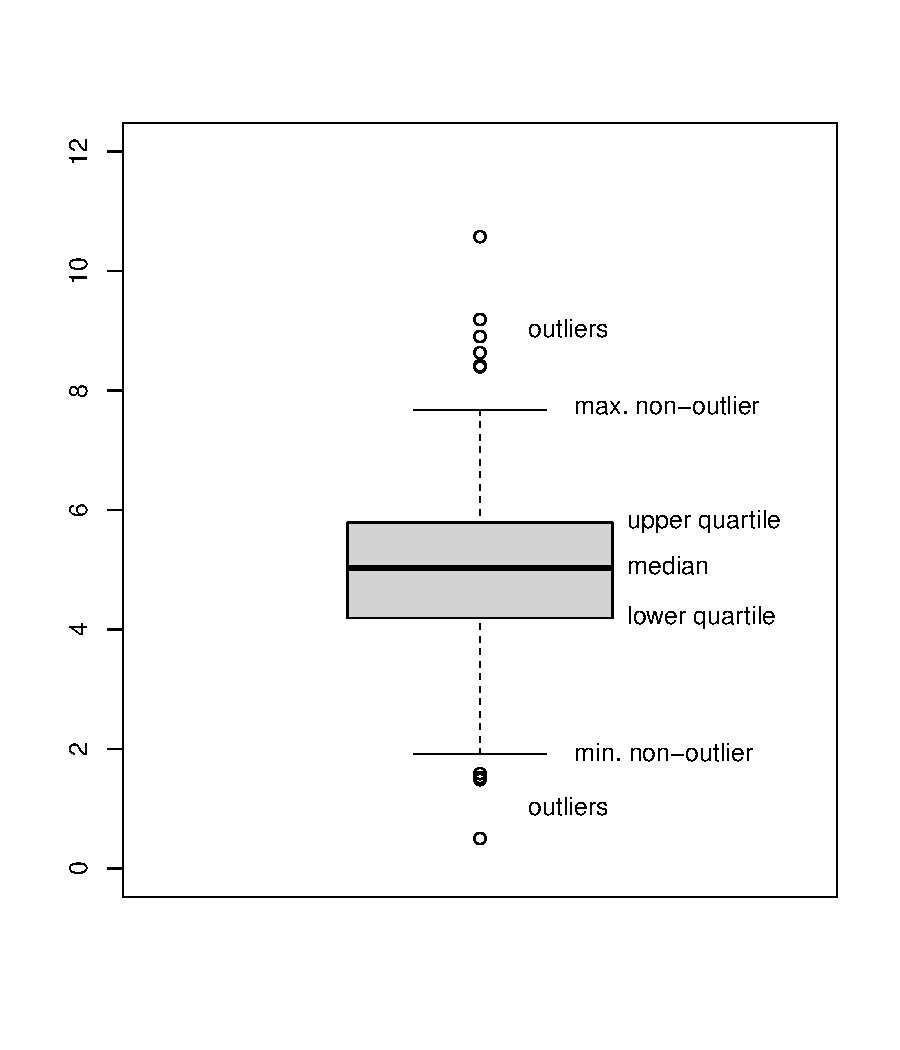
\includegraphics{math1710_files/figure-latex/boxplot1-1} \end{center}

Here are two boxplots from the July and October temperature data. What do you conclude about the data from these boxplots?

\begin{Shaded}
\begin{Highlighting}[]
\FunctionTok{boxplot}\NormalTok{(jul}\SpecialCharTok{$}\NormalTok{temp, oct}\SpecialCharTok{$}\NormalTok{temp,}
        \AttributeTok{names =} \FunctionTok{c}\NormalTok{(}\StringTok{"July"}\NormalTok{, }\StringTok{"October"}\NormalTok{),}
        \AttributeTok{ylab =} \StringTok{"Daily maximum temperature (degrees C) in Leeds"}\NormalTok{)}
\end{Highlighting}
\end{Shaded}

\begin{center}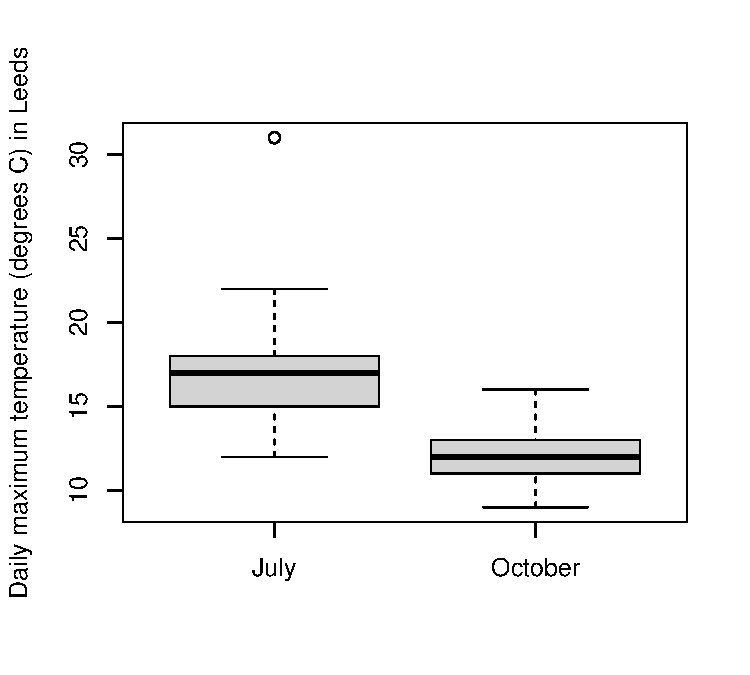
\includegraphics{math1710_files/figure-latex/boxplot-temp-1} \end{center}

(And yes, I \href{https://www.metoffice.gov.uk/binaries/content/assets/metofficegovuk/pdf/weather/learn-about/uk-past-events/interesting/2020/2020_05_july_temperature.pdf}{did check the outlier} to make sure it was a genuine datapoint.)

\hypertarget{binned}{%
\section{Binned data and histograms}\label{binned}}

Often when collecting data, we don't collect exact data, but rather collect data clumped into ``bins''. For example, suppose a student wished to use a questionnaire to collect data on how long it takes people to reach campus from home; they might not ask ``Exactly how long does it take?'', but rather give a choice of tick boxes: ``0--5 minutes'', ``5--10 minutes'', and so on.

Consider the following binned data, from \(n = 100\) students:

\begin{longtable}[]{@{}ccc@{}}
\toprule
Time & Frequency & Relative frequency \\
\midrule
\endhead
0--5 minutes & 4 & 0.04 \\
5--10 minutes & 8 & 0.08 \\
10--15 minutes & 21 & 0.21 \\
15--30 minutes & 42 & 0.42 \\
30--45 minutes & 15 & 0.15 \\
45--60 minutes & 8 & 0.08 \\
60--120 minutes & 2 & 0.02 \\
\textbf{Total} & 100 & 1 \\
\bottomrule
\end{longtable}

Here the \textbf{frequency} \(f_j\) of bin \(j\) is simply the number of observations in that bin; so, for example, 42 students had journey lengths of between 15 and 30 minutes. The \textbf{relative frequency} of bin \(j\) is \(f_j/n\); that is, the proportion of the observations in that bin.

What is the median journey length? Well, we don't know exactly, but \(0.04 + 0.08 + 0.21\) is less than 0.5, while \(0.04 + 0.08 + 0.21 + 0.42\) is greater than 0.5. So we know that the median student is in the ``10--15 minute'' bin, and we can say that the median journey length is between 10 and 15 minutes.

What about the mode? The bin with the most observations in it is the ``15--30 minute'' bin. But this bin covers 15 minutes, while some of the other bins only cover 5 minutes. It would be a fairer comparison to look at the \textbf{frequency density}: the relative frequency divided by the size of the bin.

\begin{longtable}[]{@{}cccc@{}}
\toprule
Time & Frequency & Relative frequency & Frequency density \\
\midrule
\endhead
0--5 minutes & 4 & 0.04 & 0.008 \\
5--10 minutes & 8 & 0.08 & 0.016 \\
10--15 minutes & 21 & 0.21 & 0.042 \\
15--30 minutes & 42 & 0.42 & 0.028 \\
30--45 minutes & 15 & 0.15 & 0.010 \\
45--60 minutes & 8 & 0.08 & 0.005 \\
60--120 minutes & 2 & 0.02 & 0.0003 \\
\textbf{Total} & 100 & 1 & \\
\bottomrule
\end{longtable}

In the first row, for example, the relative frequency is 0.04 and the size of the bin is 5 minutes, so the frequency density is \(0.04/5 = 0.008\). So the modal bin -- the bin with the highest frequency \emph{density} -- is in fact the ``10--15 minutes'' bin.

Since we don't have the exact data, it's not possible to exactly calculate the mean and variance. However, we can often get a good estimate by assuming that each observation was in fact right in the centre of its bin. So, for example, we can assume that all 4 observations in the ``0--5 minutes'' bin were journeys of exactly 2.5 minutes. Of course, this isn't true (or is highly unlikely to be true), but we can often get a good approximation this way.

For our journey-time data, our approximation of the mean would be
\[ \bar x = \frac{1}{100} \big(4\times 2.5 + 8 \times 7.5 + \cdots + 2\times90) = 24.4 . \]
More generally, if \(m_j\) is the midpoint of bin \(j\) and \(f_j\) its frequency, then we can calculate the binned mean and binned variance by
\begin{align*}
  \bar x &= \frac{1}{n} \sum_j f_j m_j \\
  s^2_x  &= \frac{1}{n-1} \sum_j f_j (m_j - \bar x)^2
\end{align*}

Data in bins can be illustrated with a \textbf{histogram}. A histogram has the measurement on the x-axis, with one bar across the width of each bin, with bars drawn up to the height of the corresponding frequency density. Note that this means that the area of the bar is exactly the relative frequency of the corresponding bin. (If all the bins are the same width, frequency density is directly proportional to frequency and to relative frequency, so it can be clearer use one of those as the y-axis instead.)

Here is a histogram for our journey-time data:

\begin{Shaded}
\begin{Highlighting}[]
\NormalTok{journeys }\OtherTok{\textless{}{-}} \FunctionTok{read.csv}\NormalTok{(}\StringTok{"https://mpaldridge.github.io/math1710/data/journeys.csv"}\NormalTok{)}
\NormalTok{bins }\OtherTok{\textless{}{-}} \FunctionTok{c}\NormalTok{(}\DecValTok{0}\NormalTok{, }\DecValTok{5}\NormalTok{, }\DecValTok{10}\NormalTok{, }\DecValTok{15}\NormalTok{, }\DecValTok{30}\NormalTok{, }\DecValTok{45}\NormalTok{, }\DecValTok{60}\NormalTok{, }\DecValTok{120}\NormalTok{)}

\FunctionTok{hist}\NormalTok{(journeys}\SpecialCharTok{$}\NormalTok{midpoint, }\AttributeTok{breaks =}\NormalTok{ bins,}
     \AttributeTok{xlab =} \StringTok{"Journey length (min)"}\NormalTok{,}
     \AttributeTok{main =} \StringTok{""}\NormalTok{)}
\end{Highlighting}
\end{Shaded}

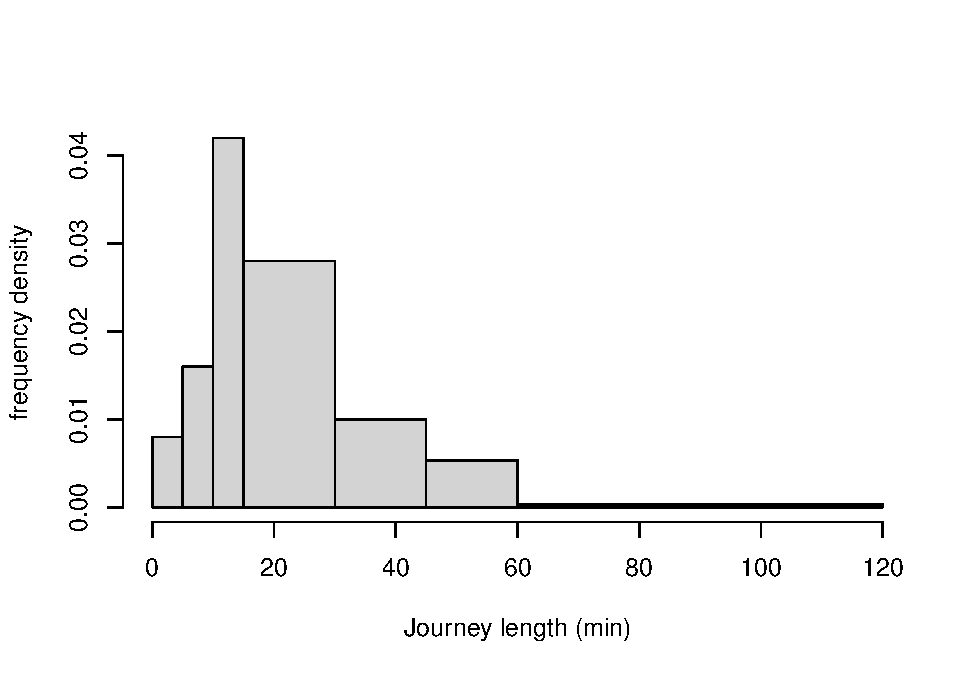
\includegraphics{math1710_files/figure-latex/journeys-1.pdf}

Often we draw histograms because the data was collected in bins. But even when we have exact data, we might choose to divide it into bins for the purposes of drawing a histogram. In this case we have to decide where to put the ``breaks'' between the bins. Too many breaks too close together, and the small number of observations in each bin will give ``noisy'' results (see left); too few breaks too far apart, and the histogram will lose detail (see right).

\begin{Shaded}
\begin{Highlighting}[]
\NormalTok{hist\_data }\OtherTok{\textless{}{-}} \FunctionTok{c}\NormalTok{(}\FunctionTok{rnorm}\NormalTok{(}\DecValTok{30}\NormalTok{, }\DecValTok{8}\NormalTok{, }\DecValTok{2}\NormalTok{), }\FunctionTok{rnorm}\NormalTok{(}\DecValTok{40}\NormalTok{, }\DecValTok{12}\NormalTok{, }\DecValTok{3}\NormalTok{))  }\CommentTok{\# Some fake data}
\FunctionTok{hist}\NormalTok{(hist\_data, }\AttributeTok{breaks =} \DecValTok{40}\NormalTok{, }\AttributeTok{main =} \StringTok{"Too many bins"}\NormalTok{)}
\FunctionTok{hist}\NormalTok{(hist\_data, }\AttributeTok{breaks =} \DecValTok{3}\NormalTok{,  }\AttributeTok{main =} \StringTok{"Too few bins"}\NormalTok{)}
\end{Highlighting}
\end{Shaded}

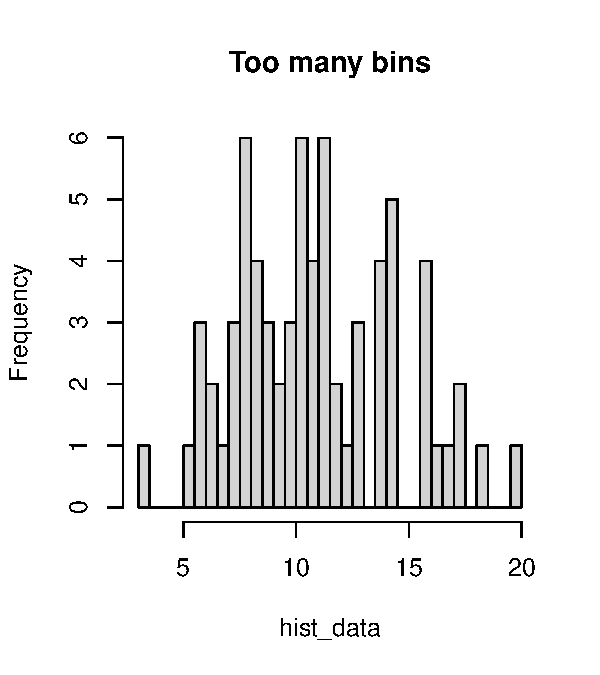
\includegraphics[width=0.48\linewidth]{math1710_files/figure-latex/hist-bins-1} 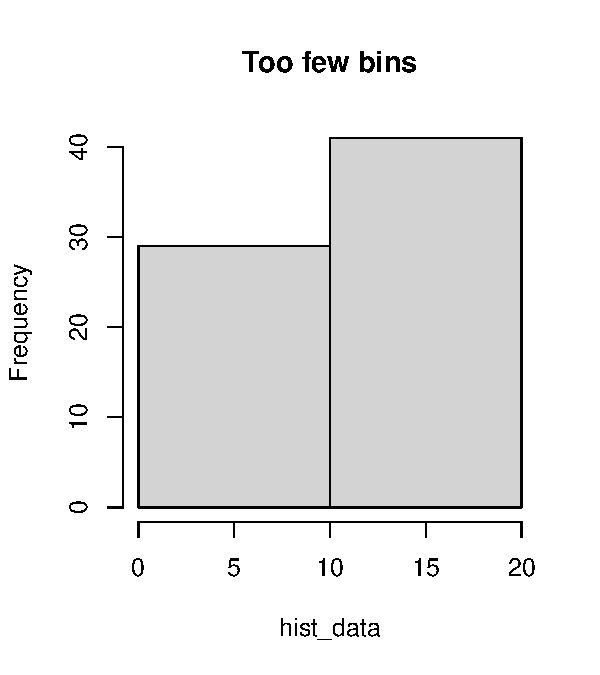
\includegraphics[width=0.48\linewidth]{math1710_files/figure-latex/hist-bins-2}

\hypertarget{multiple}{%
\section{Multiple variables and scatterplots}\label{multiple}}

Often, more than one piece of data is collected from each subject, and we wish to compare that data, to see if there is a relationship between the variables.

For example, we could take \(n\) second-year maths students, and for each student \(i\), collect their mark \(x_i\) in MATH1710 and their mark \(y_i\) in MATH1712. This gives is two ``paired'' datasets, \(\mathbf x = (x_1, x_2, \dots, x_n)\) and \(\mathbf y = (y_1, y_2, \dots, y_n)\). We can calculate sample statistics of draw plots for \(\mathbf x\) and for \(\mathbf y\) individually. But we might also want to see if there is a relationship \emph{between} \(\mathbf x\) and \(\mathbf y\): Do students with high marks in MATH1710 also get high marks in MATH1712?

A good way to visualise the relationship between two variables is to use a \textbf{scatterplot}. In a scatterplot, the \(i\)th data pair \((x_i, y_i)\) is illustrated with a mark (such as a circle or cross) whose x-coordinate has the value \(x_i\) and whose y-coordinate has the value \(y_i\).

In the following scatterplot, we have \(n = 50\) datapoints for the 50 US states; for each state \(i\), \(x_i\) is the Republican share of the vote in that state in the 2016 Trump--Clinton presidential election, and \(y_i\) is the Republican share of the vote in that state in the 2020 Trump--Biden election.

\begin{Shaded}
\begin{Highlighting}[]
\NormalTok{elections }\OtherTok{\textless{}{-}} \FunctionTok{read.csv}\NormalTok{(}\StringTok{"https://mpaldridge.github.io/math1710/data/elections.csv"}\NormalTok{)}

\FunctionTok{plot}\NormalTok{(elections}\SpecialCharTok{$}\NormalTok{X2016, elections}\SpecialCharTok{$}\NormalTok{X2020,}
     \AttributeTok{col =} \StringTok{"blue"}\NormalTok{,}
     \AttributeTok{xlab =} \StringTok{"Republican share of the two{-}party vote, 2016 (\%)"}\NormalTok{,}
     \AttributeTok{ylab =} \StringTok{"Republican share of the two{-}party vote, 2020 (\%)"}\NormalTok{)}

\FunctionTok{abline}\NormalTok{(}\AttributeTok{h =} \DecValTok{50}\NormalTok{, }\AttributeTok{col =} \StringTok{"grey"}\NormalTok{)}
\FunctionTok{abline}\NormalTok{(}\AttributeTok{v =} \DecValTok{50}\NormalTok{, }\AttributeTok{col =} \StringTok{"grey"}\NormalTok{)}
\FunctionTok{abline}\NormalTok{(}\FloatTok{0.195}\NormalTok{, }\FloatTok{0.963}\NormalTok{, }\AttributeTok{col =} \StringTok{"red"}\NormalTok{)}
\end{Highlighting}
\end{Shaded}

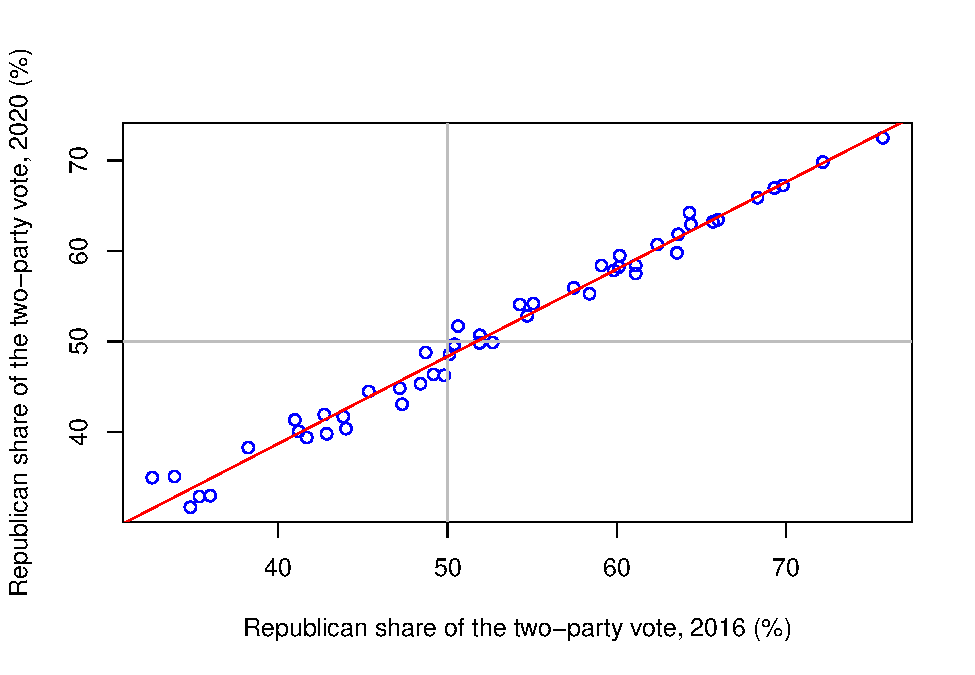
\includegraphics{math1710_files/figure-latex/elections-1.pdf}

We see that there is a strong relationship between \(\mathbf x\) and \(\mathbf y\), with high values of \(x\) corresponding to high values of \(y\) and vice versa. Further, the points on the scatterplot lie very close to a straight line.

A useful summary statistic here is the \textbf{correlation}
\[ r_{xy} = \frac{s_{xy}}{s_x s_y} , \]
where \(s_{xy}\) is the \textbf{sample covariance}
\[ s_{xy} = \frac{1}{n} \sum_{i=1}^n (x_i - \bar x)(y_i - \bar y) , \]
and \(s_x\) and \(s_y\) are the standard deviations.

The correlation \(r_{xy}\) is always between \(-1\) and \(+1\). Values of \(r_{xy}\) near \(+1\) indicate that the scatterpoints are close to a straight line with an upward slope (big \(x\) = big \(y\)); values of \(r_{xy}\) near \(-1\) indicate that the scatterpoints are close to a straight line with a downward slope (big \(x\) = small \(y\)); and values of \(r_{xy}\) near 0 indicate that there is a weak linear relationship between \(x\) and \(y\).

For the elections data, the correlation is

\begin{Shaded}
\begin{Highlighting}[]
\FunctionTok{cor}\NormalTok{(elections}\SpecialCharTok{$}\NormalTok{X2016, elections}\SpecialCharTok{$}\NormalTok{X2020)}
\end{Highlighting}
\end{Shaded}

\begin{verbatim}
## [1] 0.9919659
\end{verbatim}

which, as we expected, is extremely high.

\hypertarget{summary-01}{%
\section*{Summary}\label{summary-01}}
\addcontentsline{toc}{section}{Summary}

\begin{itemize}
\tightlist
\item
  Exploratory data analysis is about taking a first look at data.
\item
  Summary statistics are numbers calculated from data that give us useful information about the data.
\item
  Summary statistics that measure the centre of the data include the mode, median, and mean.
\item
  Summary statistics that measure the spread of the data include the number of distinct outcomes, the interquartile range, and the sample variance.
\item
  A summary statistic that measures the linear relationship between two variables is the correlation.
\item
  Boxplots, histograms, and scatterplots are useful ways of visualising data.
\end{itemize}

\hypertarget{P1}{%
\chapter*{Problem Sheet 1}\label{P1}}
\addcontentsline{toc}{chapter}{Problem Sheet 1}

This is Problem Sheet 1, which covers material from \protect\hyperlink{S01-eda}{Section 1} of the notes. You should work through all the questions on this problem sheet during Week 1, in preparation for your tutorial in Week 2. Questions C1 and C2 are assessed questions, and are due in by \textbf{2pm on Monday 11 October}. I recommend spending about 3 hours on this problem sheet in Week 1, plus 1 extra hour in Week 2 to neatly write up and submit your answers to the assessed questions.

\hypertarget{P1-short}{%
\section*{A: Short questions}\label{P1-short}}
\addcontentsline{toc}{section}{A: Short questions}

The first two questions are \textbf{short questions}, which are intended to be mostly not too difficult. Short questions usually follow directly from the material in the notes. Here, your should clearly state your final answer, and give enough working-out (or a short written explanation) for it to be clear how you reached that answer. You can check your answers with the solutions-without-working at the bottom of this sheet; solutions-with-working will be available later. If you get stuck on any of these questions, you might want to ask for guidance in your tutorial.

\textbf{A1.} Consider again the ``number of Skittles in each packet'' data from Example 1.1.
\[ 59, \ 59, \ 59, \ 59, \ 60, \ 60, \ 60, \ 61, \ 62, \ 62, \ 62, \ 63, \ 63 .\]

\textbf{(a)} Calculate the mean number of Skittles in each packet.

\textbf{(b)} Calculate the sample variance using the computational formula.

\textbf{(c)} Calculate the sample variance using the definitional formula.

\textbf{(d)} Out of (b) and (c), which calculation did you find easier, and why?

\textbf{A2.} Consider the following data sets of the age of elected politicians on a local council. (The ``18--30'' consists of people older than and including 18, and younger than but \emph{not} including 30.)

\begin{longtable}[]{@{}cccc@{}}
\toprule
Age (years) & Frequency & Relative frequency & Frequency density \\
\midrule
\endhead
18--30 & 1 & & \\
30--40 & 3 & & \\
40--45 & 4 & & \\
45--50 & 5 & & \\
50--55 & 3 & & \\
55--60 & 1 & & \\
60--70 & 3 & & \\
\textbf{Total} & 20 & 1 & --- \\
\bottomrule
\end{longtable}

\textbf{(a)} Complete the table by filling in the relative frequency and frequency densities.

\textbf{(b)} What is the median age bin?

\textbf{(c)} Calculate (an approximation of) the mean age of the politicians.

\hypertarget{P1-long}{%
\section*{B: Long questions}\label{P1-long}}
\addcontentsline{toc}{section}{B: Long questions}

The next four questions are \textbf{long questions}, which are intended to be harder. Long questions often require you to think originally for yourself, not just directly follow procedures from the notes. Here, your answers should be written in complete sentences, and you should carefully explain in words each step of your working. Your answers to these questions -- not only their mathematical content, but also how to clearly write good solutions -- are likely to be the main topic for discussion in your tutorial.

\textbf{B1.} For each of the two datasets below, calculate the following summary statistics, or explain why it is not possible to do so: mode; median; mean; number of distinct outcomes; inter-quartile range; and sample variance.

\textbf{(a)} Six packets of Skittles are opened together, and the total number of sweets of each colour is:

\begin{longtable}[]{@{}cccccc@{}}
\toprule
\textbf{Colour} & Red & Orange & Yellow & Green & Purple \\
\midrule
\endhead
\textbf{Number of Skittles} & 67 & 71 & 87 & 74 & 62 \\
\bottomrule
\end{longtable}

\textbf{(b)} Shirt sizes for a university football squad:

\begin{longtable}[]{@{}cccccc@{}}
\toprule
\textbf{Colour} & Xtra Small & Small & Medium & Large & Xtra Large \\
\midrule
\endhead
\textbf{Number of Skittles} & 0 & 1 & 6 & 5 & 4 \\
\bottomrule
\end{longtable}

\textbf{B2.} A summary statistic is informally said to be ``robust'' if it typically doesn't change much if a small number of outliers are introduced to a large dataset, or ``sensitive'' if it often changes a lot when a small number of outliers are introduced. Briefly discuss the robustness or sensitivity of the following summary statistics: \textbf{(a)} mode; \textbf{(b)} median; \textbf{(c)} mean; \textbf{(d)} number of distinct outcomes; \textbf{(e)} inter-quartile range; and \textbf{(f)} sample variance.

\textbf{B3.} Let \(\mathbf a = (a_1, a_2, \dots a_n)\) and \(\mathbf b = (b_1, b_2, \dots, b_n)\) be two real-valued vectors of the same length. Then the \emph{Cauchy--Schwarz inequality} says that
\[ \left( \sum_{i=1}^n a_i b_i \right)^2 \leq \left( \sum_{i=1}^n a_i^2 \right) \left(\sum_{i=1}^n b_i^2 \right) . \]
Use the Cauchy--Schwarz inequality to show that the correlation \(r_{xy}\) satisfies \(-1 \leq r_{xy} \leq 1\).

(\emph{Hint:} Try to prove that \(s_{xy}^2 \leq s_x^2 s_y^2\). How does this help?)

\textbf{B4.} A researcher wishes to study the effect of mental health on academic achievement. The researcher will collect data on the mental health of a cohort of students by asking them to fill in a questionnaire, and will measure academic achievement via the students' scores on their university exams. Discuss some of the ethical issues associated with the collection, storage, and analysis of this data, and with the publication of the results of the analysis. Are there ways to mitigate these issues?

(It's not necessary to write an essay for this question -- a few short bulletpoints will suffice. There may be an opportunity to discuss these issues in more detail in your tutorial.)

\hypertarget{P1-assessed}{%
\section*{C: Assessed questions}\label{P1-assessed}}
\addcontentsline{toc}{section}{C: Assessed questions}

The last two questions are \textbf{assessed questions}. This means you will submit your answers, and your answers will be marked by your tutor. These two questions count for 3\% of your final mark for this module. If you get stuck, your tutor may be willing to give you a hint in your tutorial.

The deadline for submitting your solutions is \textbf{2pm on Monday 11 October} at the beginning of Week 3, although I strongly recommend completing and submitting your work during Week 2. Submission will be via Gradescope; submission will open on Monday 4 October.
You should submit your answers as a single PDF file. Most students choose to hand-write their work, then scan it to PDF using their phone; if you do this, you should use a proper scanning app (like Microsoft Lens or Adobe Scan) -- please do not just submit photographs. We will discuss Gradescope submission further in the Week 2 lectures. Your work will be marked by your tutor and returned on Monday 18 September, when solutions will also be made available.

Question C1 is a ``short question'', where brief explanations or working are sufficient; Question C2 is a ``long question'', where the marks are not only for mathematical accuracy but also for the clarity and completeness of your explanations.

You should not collaborate with others on the assessed questions: your answers must represent solely your own work. The University's rules on \href{https://library.leeds.ac.uk/info/1401/academic_skills/46/academic_integrity_and_plagiarism}{academic integrity} -- and the related punishments for violating them -- apply to your work on the assessed questions.

\textbf{C1.} The monthly average exchange rate for US dollars into British pounds over a 12-month period was:
\begin{gather*}
1.306, \ 1.301, \ 1.290, \ 1.266, \ 1.290, \ 1.302,\\
1.317, \ 1.304, \ 1.284, \ 1.268, \ 1.247, \ 1.215.
\end{gather*}

\textbf{(a)} Calculate the median for this data.

\textbf{(b)} Calculate the mean for this data.

\textbf{(c)} Calculate the sample variance for this data.

\textbf{(d)} Is the mode an appropriate summary statistic for this data? Why/why not?

\textbf{C2.}
~\textbf{(a)} Prove the following computational formula for the sample covariance:
\[ s_{xy} = \frac{1}{n-1} \left( \sum_{i=1}^n x_iy_i - n\bar x \bar y \right). \]

\textbf{(b)} Suppose that a dataset \(\mathbf x = (x_1, x_2, \dots, x_n)\) (with \(n \geq 2\)) has sample variance \(s_x^2 = 0\). Show that all the datapoints are in fact equal.

\hypertarget{P1-short-sols}{%
\section*{Solutions to short questions}\label{P1-short-sols}}
\addcontentsline{toc}{section}{Solutions to short questions}

\textbf{A1.} (a) 60.7 (b) \& (c) 2.40 (d) ---

\textbf{A2.} (a) --- (b) 45--50 (c) 47.3

\hypertarget{part-other-stuff}{%
\part*{Other stuff}\label{part-other-stuff}}
\addcontentsline{toc}{part}{Other stuff}

\hypertarget{R}{%
\chapter*{R Worksheets}\label{R}}
\addcontentsline{toc}{chapter}{R Worksheets}

\hypertarget{r-work}{%
\section*{R worksheets}\label{r-work}}
\addcontentsline{toc}{section}{R worksheets}

Each week there will be an R worksheet to work through in your own time. We recommend spending about one hour on each worksheet, plus one extra hour for worksheets with assessed questions, for checking through and submitting your solutions.

\begin{longtable}[]{@{}clc@{}}
\toprule
Week & Worksheet & Deadline for assessed work \\
\midrule
\endhead
1 & \href{https://mpaldridge.github.io/math1710/R1.html}{\textbf{R basics}} & --- \\
2 & Working with vectors & --- \\
3 & Importing data into R & Monday 18 October \\
4 & Plots I: Making plots & --- \\
5 & Plots II: Making plots nicer & Monday 1 November \\
6 & RMarkdown (optional) & --- \\
7 & Discrete random variables & Monday 15 November \\
8 & Discrete distributions & --- \\
9 & Normal distribution & Monday 29 November \\
10 & Law of large numbers & --- \\
11 & Summary & \emph{To be confirmed} \\
\bottomrule
\end{longtable}

\hypertarget{about-r}{%
\section*{About R and RStudio}\label{about-r}}
\addcontentsline{toc}{section}{About R and RStudio}

\begin{itemize}
\tightlist
\item
  \textbf{R} is a \emph{programming language} that is particularly good at working with probability and statistics. R is very widely used in universities and increasingly widely used in industry. Learning to use R is a mandatory part of this module, and exercises requiring use of R make up at least 15\% of your module mark. Many other statistics-related course at the University also use R.
\item
  \textbf{RStudio} is a \emph{program} that gives a convenient way to work with the language R. RStudio is the most common way to use the language R, and learning to use RStudio is strongly recommended.
\end{itemize}

R and RStudio are free/open-source software.

\hypertarget{r-access}{%
\section*{How to access R and RStudio}\label{r-access}}
\addcontentsline{toc}{section}{How to access R and RStudio}

There are a number of ways you can access R and RStudio:

\begin{itemize}
\tightlist
\item
  All \textbf{University computers} have R and RStudio already installed. \href{https://it.leeds.ac.uk/it/?id=kb_article\&sysparm_article=KB0013658}{Here is a directory of the University's computer clusters.}
\item
  You can \textbf{install} R and RStudio on your own computer -- see the instructions below.
\item
  If you want to use R/RStudio on a non-University device for which you don't have admin/installation rights (Chromebook, iPad, friend's laptop, etc), you could try:

  \begin{itemize}
  \tightlist
  \item
    You can use the University's copies of R/RStudio virtually through the \href{https://it.leeds.ac.uk/it?id=kb_article\&sysparm_article=KB0014379}{Windows Virtual Desktop} or \href{https://it.leeds.ac.uk/it?id=kb_article\&sysparm_article=KB0014827}{AppsAnywhere} client.
  \item
    The \href{https://rstudio.cloud/}{RStudio Cloud} is a cloud-hosted ``Google Docs for R'' that you can use through your web browser -- you can get 25 hours per month for free (or pay for more).
  \end{itemize}
\end{itemize}

\hypertarget{r-install}{%
\section*{Installing R and RStudio}\label{r-install}}
\addcontentsline{toc}{section}{Installing R and RStudio}

Students who have their own computer usually find it most convenient to install R and RStudio on that computer. To do this, it's important that you install R (the programming language) first, and only install RStudio (the program to use R) once R has already been installed.

\begin{enumerate}
\def\labelenumi{\arabic{enumi}.}
\item
  \emph{First}, install \textbf{R}. Go to the \href{https://cran.r-project.org/}{Comprehensive R Archive Network} and follow the instructions:

  \begin{itemize}
  \tightlist
  \item
    Windows: Click \href{https://cran.r-project.org/bin/windows/}{``Download R for Windows''}, then \href{https://cran.r-project.org/bin/windows/base/}{``Install R for the first time''}. The main link at the top should be to download the most recent version of R.
  \item
    Mac: Click \href{https://cran.r-project.org/bin/macosx/}{Download R for macOS}, and then download the relevant PKG file. (For pre-November 2020 Intel-based Macbooks, you must use the ``Intel 64-bit build''; for post-November 2020 M1-based ``Apple silicon'' Macbooks, the ``Apple silicon arm64 build'' may be faster.)
  \end{itemize}
\item
  \emph{After} R is installed, \emph{then} install \textbf{RStudio}. Go to \href{https://www.rstudio.com/products/rstudio/download/\#download}{the Download page at RStudio.com} and follow the instructions. You want ``RStudio Desktop'', and you want the free version.
\end{enumerate}

If you have difficulty installing R, come along to the first computational drop-in session in Week 2 and bring your computer with you (if it's sufficiently portable), and we'll do our best to help.

\hypertarget{troubleshooting}{%
\section*{Troubleshooting drop-in sessions}\label{troubleshooting}}
\addcontentsline{toc}{section}{Troubleshooting drop-in sessions}

You will learn to use R by working through the R Worksheets. Learning to use a programming language is different from learning mathematics: you should expect to regularly get frustrated and annoyed when the computer seems to refuse to do what you want it to (but also occasionally experience the joy of getting it right!). This is a normal part of learning.

However, many students find getting with started with R in the first few weeks particularly frustrating. Also, sometimes students have problems installing R and RStudio on their own computers. To help with this, we have organised optional troubleshooting drop-in sessions in Weeks 2 and 3. Check your timetable for details -- they are probably listed as ``computer practicals''.

\end{document}
